\label{sec:hadhad_multijet}

Multi-jet production represents a relevant source of background in the
\hadhad signal region, with both \tauhadvis candidates originating
from the misidentification of quark- or gluon-initiated jets. It
represents the second largest background with \faketauhadvis in the
\hadhad SR after the dominant \ttbarFakes contribution.

The multi-jet background is estimated using the fake factor method
which is a data-driven method for background estimation. The method is
applicable in cases where two observables exist that are statistically
independent for the background process, while also being strong
discriminators between the background process of interest and more
signal-like events. Four disjoint regions can be defined, three
background-enriched CRs and a SR, by applying selections on both
observables. The independence assumption allows to relate the observed
number of background events in the three CRs with the background
expectation in the SR, yielding data-driven estimate of the background
in the SR.

In the \hadhad channel two observables allowing to define multi-jet
enriched control regions are the \tauid requirements applied to
\tauhadvis candidates and the sign of the electric charges of both
candidates.

In the \hadhad SR, \tauhadvis candidates are required to pass the
loose \tauid working point. The regions defined by this requirement
are herafter called the ID regions. This \tauid requirement is
(partially) inverted to obtain a region enhanced in multi-jet events
by requiring that exactly one \tauhadvis fails the loose \tauid
working point, still fulfilling a very loose working point
corresponding to a percent level efficiency loss in true \tauhad
($\text{RNN score} > 0.01$). The regions defined according to these
requirements are herafter referred to as Anti-ID regions. The ID
requirements cannot be fully inverted due to selections applied for
data reduction in the ATLAS experiment in datasets targeting
$\PHiggs \to \hadhad$ where at least one \tauhadvis is required to
pass the loose working point and both \tauhadvis fulfilling
$\text{RNN score}$ > 0.01.\todo{Maybe say that this is not really a
  problem?}

The electric charge of both \tauhadvis candidates produced from the
signal processes and dominant sources of backgrounds with two
\tauhadvis orginating for hadronic $\tau$~decays ($\PZ \to \tautau$,
$\PHiggs \to \tautau$, \ttbar) are expected to be reconstructed with
opposite sign (OS) electric charge. The OS requirement is inverted
yielding regions with \tauhadvis candidates of same sign (SS) electric
charge that are depleted of processes where both \tauhadvis orginate
from hadronic $\tau$ decays. The multi-jet background is expected to
contribute similarly to the OS and SS regions since the \tauhadvis
charge reconstruction is not very sensitive to the charge of the
partons initiating the jets.

With the previously defined control regions and assumption of
independence of both categorical observables, the expected multi-jet
contribution in regions with \tauhadvis passing loose identification
and opposite-sign electric charge can be estimated using
\begin{align*}
  N_\text{multi-jet}^{\text{OS, ID}} =
  N_\text{multi-jet}^{\text{OS, Anti-ID}}
  \cdot
  \underbrace{\frac{N_\text{multi-jet}^{\text{SS, ID}}}
                   {N_\text{multi-jet}^{\text{SS, Anti-ID}}}}
  _{\text{FF}_\text{SS}} \,\text{,}
  \label{eq:ff_method}
\end{align*}
where $N_\text{multi-jet}$ is the number of multi-jet events in a
given region. The fake factor (FF) measures the ratio of multi-jet
events in the ID and Anti-ID region\footnote{For the fake factor
  method one observable (the one that form the ratio of the fake
  factors...) is related to identification or isolation criteria of
  reconstructed physics objects, distinuishing it from the more
  general ABCD method.}. \todo{Differential description...}

The previously defined control regions do not provide a pure sample of
multi-jet events thus $N_\text{multi-jet}$ needs to be estimated
separately. The number of multi-jet events is estimated by subtracting
from the number of observed events ($N_\text{data}$), the expected
number of non-multi-jet events ($N_\text{non-multi-jet}$) estimated
using Monte Carlo simulation, i.e.\
$N_\text{multi-jet} = N_\text{data} - N_\text{non-multi-jet}$.

In~\Cref{tab:mjfakes_yields} the multi-jet and non-multi-jet yields in
the regions relevant for the \faketauhadvis estimation are
summarised. The 2 $b$-tag region is not well suited to estimate the
fake factors:
\begin{itemize}
\item The regions entering the fake factor measurement have a sizable
  contamination from non-multi-jet backgrounds that have to be
  subtracted. The primary source of non-multi-jet background is
  \ttbarFakes.

\item The \btag requirement strongly suppresses the multi-jet
  contribution leading to large statistical uncertainties on the
  estimated fake factors, preventing differential measurements of fake
  factors.

\item The absence of a 2 $b$-tag multi-jet validation region prevents
  validation the multi-jet estimate obtained with the fake factor
  method. Moreover, the independence of the charge sign and ID
  observables used for the FF method cannot be checked.
\end{itemize}

\begin{table}[htbp]
  \centering

  \begin{subtable}[t]{\textwidth}
    \centering
    % Size of subtraction and multi-jet purity:
%                         multi_jet  non_multi_jet  multi_jet_error  non_multi_jet_error  multi_jet_purity
% anti_id charge_sign
% False   OS           16067.048497   16443.951503       204.558258            96.607872          0.494203
%         SS           14040.394005    1971.605995       129.147367            25.827164          0.876867
% True    OS           91582.182374   13677.817626       334.090987            79.729466          0.870057
%         SS           78399.983641    5707.016359       296.470480            61.544664          0.932146

\begin{tabular}{
  ll
  S[table-format=5.0(3)]
  S[table-format=5.0(3)]
  c}
  \toprule
  \multicolumn{2}{l}{Region} & {$N_\text{multi-jet}$} & {$N_\text{non-multi-jet}$} & {Multi-jet purity} \\
  \midrule
  \multirow{2}{*}{SS} & ID      & 14040 +- 130 & 1970 +- 30   & 88\,\% \\
                      & Anti-ID & 78400 +- 300 & 5710 +- 70   & 93\,\% \\
  \midrule
  \multirow{2}{*}{OS} & ID      & 16070 +- 210 & 16440 +- 100 & 49\,\% \\
                      & Anti-ID & 91580 +- 340 & 13680 +- 80  & 87\,\% \\
  \bottomrule
\end{tabular}



%%% Local Variables:
%%% mode: latex
%%% TeX-master: "../phd_thesis"
%%% End:

    \subcaption{1 $b$-tag regions}
  \end{subtable}

  \begin{subtable}[t]{\textwidth}
    \centering
    % Size of subtraction and multi-jet purity:
%                        multi_jet  non_multi_jet  multi_jet_error  non_multi_jet_error  multi_jet_purity
% anti_id charge_sign
% False   OS            408.197943    7971.802057       105.950917            53.344135          0.048711
%         SS           1299.622259    1001.377741        50.345854            15.287412          0.564808
% True    OS           8429.603396    8864.396604       139.699303            47.136984          0.487429
%         SS           7653.735896    3338.264104       108.557939            28.157166          0.696301

\begin{tabular}{
  ll
  S[table-format=5.0(3)]
  S[table-format=5.0(3)]
  c}
  \toprule
  \multicolumn{2}{l}{Region} & {$N_\text{multi-jet}$} & {$N_\text{non-multi-jet}$} & {Multi-jet purity} \\
  \midrule
  \multirow{2}{*}{SS} & ID      & 1300 +- 60  & 1000 +- 20 & 56\,\% \\
                             & Anti-ID & 7650 +- 110 & 3340 +- 30 & 70\,\% \\
  \midrule
  \multirow{2}{*}{OS} & ID      & \multicolumn{3}{c}{\rule[3pt]{5.2em}{0.3pt}\hspace{1em}Signal Region\hspace{1em}\rule[3pt]{5.2em}{0.3pt}} \\
                             & Anti-ID & 8430 +- 140 & 8860 +- 50 & 49\,\% \\
  \bottomrule
\end{tabular}




%%% Local Variables:
%%% mode: latex
%%% TeX-master: "../phd_thesis"
%%% End:

    \subcaption{2 $b$-tag regions}
  \end{subtable}

  \caption{Statistical uncertainties only. The signal region (2
    $b$-tag OS ID) is omitted.}
  \label{tab:mjfakes_yields}
\end{table}

Instead use 1-tag (do not expect \btag to affect fake factor estimate)
% Dominant subtraction is ttbar, execpt for 1-tag OS ID where it is
% Ztautau.


% Can use table to prove independence:
% (ID | SS) / (Anti-ID | SS) = 17.9
% (ID | OS) / (Anti-ID | OS) = 17.5

% 1. Use 1-tag since it has higher abundance of multi-jet, less subtraction and can be used to validate independence

% Signal contamination / other background contamination

% Yield table / plots of regions


\begin{figure}[htbp]
  \centering

  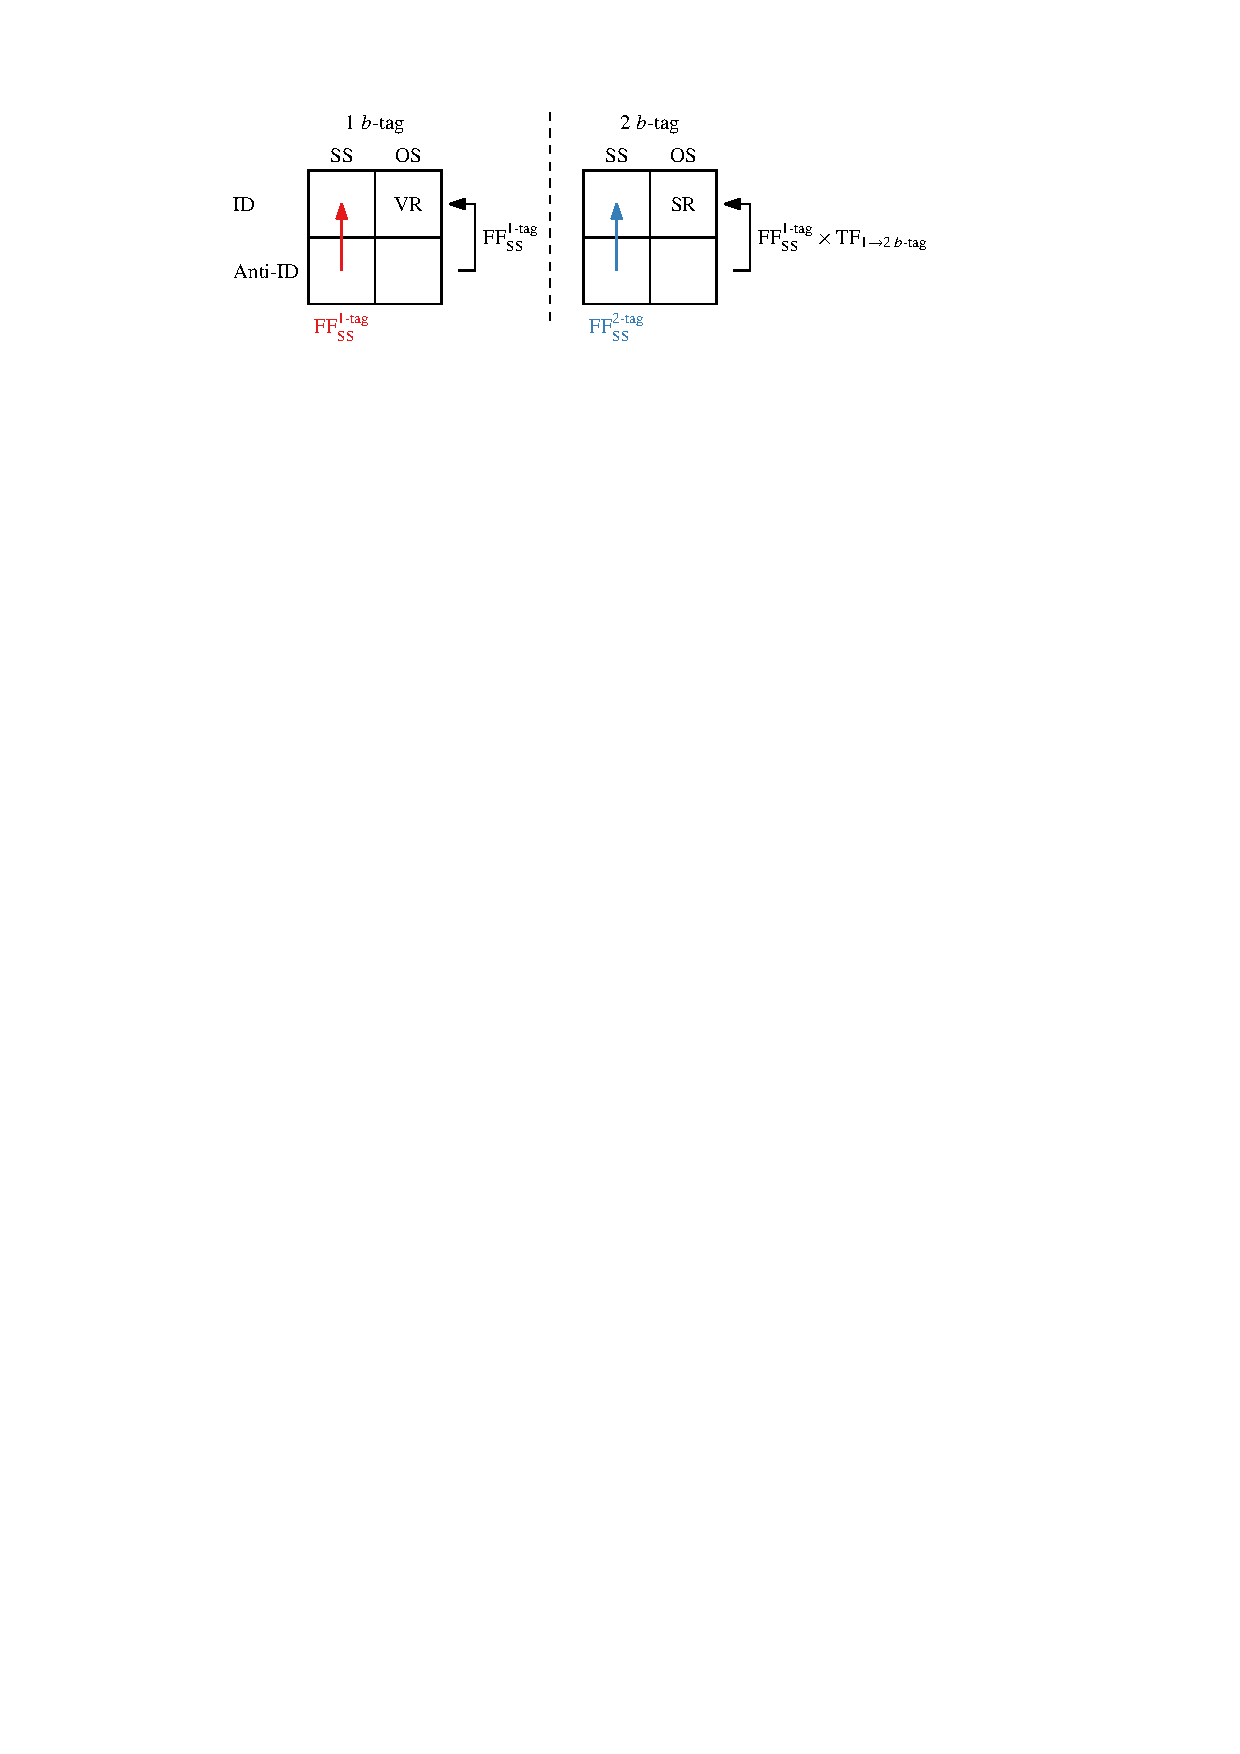
\includegraphics[scale=1]{fakefactors/regions}

  \caption{Region definitions}
  \label{fig:fakefactor_regions}
\end{figure}

% Checked in 1-tag OS. Does agreement in 1-tag OS confirm that charge
% and ID are independent? Closure, yes

The fake factor (FF) measures the ratio of events with fake \tauhadvis in ID and
Anti-ID region:
\begin{align*}
  \FF = \frac{N\left( \text{fake} \, \tauhadvis, \text{ID} \right)}{N\left( \text{fake} \, \tauhadvis, \text{Anti-ID} \right)}
\end{align*}
The probability of a jet faking a \tauhadvis depends strongly on \tauhadvis \pT
and decay mode. Therefore, the fake factor is frequently parametrised in these
quantities. It is also affected by the \tauhadvis identification already applied
in the high-level \tauhadvis-triggers which also needs to be taken into account.

The fake factors are measured in the fake enriched SS-region by subtracting
non-fake-\tauhadvis background using their estimates from simulation:
\begin{align*}
  \FF_\text{SS} = \frac{N(\text{SS}, \text{ID}) - N_\text{non-fake}(\text{SS}, \text{ID})}{N(\text{SS}, \text{Anti-ID}) - N_\text{non-fake}(\text{SS}, \text{Anti-ID})}
\end{align*}
where $N$ is the total yield and $N_\text{non-fake}$ the yield of
non-fake-\tauhadvis backgrounds in the corresponding region.

To obtain the fake \tauhadvis estimate in the OS ID-region, the assumption is
made that the fake factors are independent of the reconstructed charge of the
fake \tauhadvis candidates. Therefore, the SS fake factors $\FF_\text{SS}$ are
applied to events in the OS Anti-ID region after subtracting any
non-fake-\tauhadvis contributions.
\begin{align*}
  N(\text{fake}, \text{OS ID}) = \FF_\text{SS} \times \left[ N(\text{OS}, \text{Anti-ID}) - N_\text{non-fake}(\text{OS}, \text{Anti-ID}) \right]
\end{align*}
Systematic uncertainties are assigned to
cover possible difference betwen OS and SS fake factors, varying the
subtraction in the OS Anti-ID region. Moreover, the fake factors are
independently varied by their statistical uncertainty.

Due to the limited acceptance of fake \tauhadvis in the 2 \btag region, the 1
\btag region is used to calculate the fake factors instead. The 1 \btag fake
factors are applied to the 2 \btag OS Anti-ID region and an additional 1 to 2
\btag transfer factor is applied.

The binning of the fake factors is dependent on the trigger that selected the
event. For STT events the fake factor is binned in whether the anti-\tauhadvis
is leading or subleading in \pT, and the decay mode of the \tauhadvis
($N_\text{track}$). Due to low statistics in the STT category the fake factors
are inclusive in \tauhadvis \pT. The \tauhadvis identification at the HLT is
only applied to one of the two \tauhadvis candidates affecting the probability
of jets faking \tauhadvis, motivating the binning in whether the leading /
subleading \tauhadvis fails the identification.

For DTT events, HLT \tauhadvis identification is applied to both \tauhadvis
candidates. Therefore, the fake factors do not need to distinguish between cases
where the leading and subleading \tauhadvis fails the loose identification. The
fake factors for DTT events are parametrised in the \pT and decay mode of the
the \tauhadvis candidate failing the identification requirement.

Moreover, all fake factors are binned by data-taking period (${\text{2015-2016},
  \text{2017}, \text{2018}}$) which takes into account the different triggers
being used to select events used for the analysis.

\todo[inline]{Could we use nOS to enhance statistics? Maybe flip the FF method
  so that we use events in SS ID to build the template instead of OS Anti-ID.}

\todo[inline]{Can we make the STT FF depend on the trigger-match instead of
  the leading / subleading binning?}


%%% Local Variables:
%%% mode: latex
%%% TeX-master: "../../phd_thesis"
%%% End:
